\documentclass[12pt]{article}

\usepackage[T1]{fontenc}
\usepackage{geometry}
\usepackage{amsmath, amssymb, amsthm}
\usepackage{hyperref}
\usepackage{graphicx}
\usepackage{float}
\usepackage[titles]{tocloft}
\usepackage{enumitem}

\geometry{a4paper, margin=1in}

\setlength{\cftbeforesecskip}{1em}
\setlength{\cftbeforesubsecskip}{0.5em}
\setlength{\parskip}{1em}
\setlength{\parindent}{0em}

\setlist{nolistsep, itemsep=0.5em}


\newcommand{\N}{\mathbb{N}}
\newcommand{\Z}{\mathbb{Z}}
\newcommand{\Q}{\mathbb{Q}}
\newcommand{\R}{\mathbb{R}}
\newcommand{\C}{\mathbb{C}}


\newtheorem{theorem}{Theorem}[section]
\newtheorem{corollary}{Corollary}[theorem]
\newtheorem{lemma}[theorem]{Lemma}

\theoremstyle{definition}
\newtheorem{definition}{Definition}[section]

\theoremstyle{remark}
\newtheorem*{remark}{Remark}
\newtheorem*{example}{Example}


\title{
    The hyperbolic plane as the universal cover of the double torus
}
\author{Satvik Saha}
\date{14 July, 2022}

\begin{document}

    \begin{center}
    \vspace*{\fill}
    \thispagestyle{empty}
        \includegraphics[width=4cm]{iiserk_logo.png}

        \vspace{0.5cm}

        {
            \Large\bfseries
            Indian Institute of Science Education and Research, Kolkata\par
        }

        \vspace{0.2cm}

        {
            \large
            Department of Mathematics and Statistics
        }

        \vspace{0.1cm}

        {
            \large\it
            Summer Project Report, May-July 2022
        }

        \vspace{1cm}

        {
            \LARGE\bfseries
            The hyperbolic plane as the universal cover of the double torus\par
        }

        \vspace{1cm}

        Submitted by\\
        \vspace{0.2cm}
        {
            \Large\bfseries
            Satvik Saha
        }

        \vspace{0.8cm}

        On\\
        \vspace{0.2cm}
        {
            \Large\bfseries
            14 July, 2022
        }

        \vspace{0.8cm}

        Under the supervision of\\
        \vspace{0.2cm}
        {
            \Large\bfseries
            Dr. Somnath Basu\\
        }
        \vspace{0.2cm}
        {
            \large
            Department of Mathematics and Statistics\\
            IISER Kolkata
        }
    \vspace*{\fill}
    \end{center}

    \clearpage

    \section*{\LARGE Declaration}
    \addcontentsline{toc}{section}{\numberline{}Declaration}

    I declare here that the report included in this project entitled ``The hyperbolic
    plane as the universal cover of the double torus'' is the summer internship
    carried out by me in the Department of Mathematics and Statistics, Indian
    Institute of Science Education and Research Kolkata, India from May 17 to July
    14, 2020 under the supervision of  Dr. Somnath Basu.


    In keeping with general practice of reporting scientific observations, due
    acknowledgements have been made wherever the work described is based on the
    findings of other investigators.

    \vspace{5cm}
    \noindent
    \begin{tabular*}{\textwidth}{l@{\extracolsep{\fill}}r}
        July 14, 2022 & Satvik Saha \\
        \textbf{IISER Kolkata} &
    \end{tabular*}

    \clearpage

    \section*{\LARGE Certificate}
    \addcontentsline{toc}{section}{\numberline{}Certificate}

    It is certified that the summer research work included in the project report
    entitled ``The hyperbolic plane as the universal cover of the double torus'' has
    been carried out by Mr. Satvik Saha under my supervision and guidance. The
    content of this project report has not been submitted elsewhere for the award of
    any academic and professional degree.

    \vspace{5cm}
    \noindent
    \begin{tabular*}{\textwidth}{l@{\extracolsep{\fill}}r}
        July 14, 2022 & Dr. Somnath Basu \\
        \textbf{IISER Kolkata} & \textbf{Project Supervisor}
    \end{tabular*}

    \clearpage

    \tableofcontents
    \addcontentsline{toc}{section}{\numberline{}Contents}
    \clearpage

    \section*{\LARGE Acknowledgements}
    \addcontentsline{toc}{section}{\numberline{}Acknowledgements}

    I would like to thank Dr. Somnath Basu for his guidance and support. I also like
    to thank my friends and teammates, who made working with them this summer an
    njoyable experience.

    I sincerely thank IISER Kolkata for giving me the opportunity to carry out my
    summer internship.

    \vspace{5cm}
    \noindent
    \begin{tabular*}{\textwidth}{l@{\extracolsep{\fill}}r}
        July 14, 2022 & Satvik Saha \\
        \textbf{IISER Kolkata} &
    \end{tabular*}

    \clearpage



    \cftaddtitleline{toc}{section}{\\
            The hyperbolic plane as the universal cover of the double torus
    }{}
    \begin{center}
        {
            \LARGE\bfseries
            The hyperbolic plane as the universal cover of the double torus\par
        }
    \end{center}
    \vspace{0.2cm}

    \begin{abstract}
        We study the double torus, a compact orientable manifold $\Sigma_2$ of genus
        $2$, and its universal cover. In particular, we examine the upper half plane
        $\mathbb{H}^2$ and the Poincar\'e disc $\mathbb{D}^2$ models of the
        hyperbolic plane. We use this to compute the fundamental group of $\Sigma_2$
        and discuss its relationship with the group of deck transformations on
        $\mathbb{D}^2$. We further note that this covering space induces a metric of
        constant negative Gaussian curvature on $\Sigma_2$.
    \end{abstract}

    \section{Introduction}

    The double torus is our primary object of study. It can be described as a
    topological manifold, obtained from the connected sum of two tori. In other
    words, take two tori, remove a small open disc from both, then glue them together
    along their new boundaries. The result is a compact manifold of genus 2, which we
    refer to as $\Sigma_2$. The process of taking connected sums of tori can be
    repeated, with $n$ contributing tori yielding a compact manifold $\Sigma_g$ of
    genus $g$.

    \begin{figure}[H]
        \begin{center}
            \includegraphics[width=0.9\textwidth]{figures/tori.png}
        \end{center}
        \caption{The torus and the double torus, representing the structures
        $\Sigma_1$ and $\Sigma_2$.}
        \label{fig:tori}
    \end{figure}

    The manifold $\Sigma_2$ has many possible embeddings in the real space $\R^3$,
    and each of these induces a differential structure, hence a notion of curvature
    on the surface. In Figure.~1, we see that this representation of $\Sigma_2$ has
    regions of positive curvature where the surface bulges outwards, and regions of
    negative curvature where it caves inwards. 


    \begin{theorem}
        If $\Sigma \subseteq \R^3$ is a compact surface, then there exists a point $p
        \in \Sigma$ where the Gaussian curvature $K(p) > 0$.
    \end{theorem}
    \begin{proof}
        Consider the map \[
            f\colon \Sigma \to \R, \qquad v \mapsto \Vert v\Vert^2.
        \] From the compactness of $\Sigma$, this must attain a maximum and minimum
        at some points $p_+, p_- \in \Sigma$. At such points, we have $Df_p\equiv 0$,
        but \[
            Df_p\colon T_p\Sigma \to T_{f(p)}\R, \qquad v \mapsto 2\langle p,
            v\rangle.
        \] Thus, we must have $p_{\pm} \perp T_{p_\pm}\Sigma$. Now, pick a regular
        curve $\gamma$ in $\Sigma$ based at $p_+$. Then $f\circ \gamma$ must attain
        its maximum at $0$, hence \[
            \frac{d}{dt}f(\gamma(t))\Big|_{t = 0} = 0, \qquad
            \frac{d^2}{dt^2}f(\gamma(t))\Big|_{t = 0} \leq 0.
        \] This means that \[
            2\langle \gamma(0), \dot{\gamma}(0)\rangle = 0, \qquad
            2[\Vert \dot{\gamma}(0) \Vert^2 + \langle \gamma(0),
            \ddot{\gamma}(0)\rangle] \leq 0.
        \] By construction, $\Vert \dot{\gamma}\Vert = 1$, $\gamma(0) = p_+$, and
        $\Vert \ddot{\gamma}(0)\Vert$ is the curvature $\kappa$. The latter
        inequality gives $\kappa \geq 1 / \Vert p_+ \Vert$. Since this is true for
        any such $\gamma$, this must also hold for the principal curvatures $k_1,
        k_2$, hence the Gaussian curvature $K(p_+) = k_1k_2 \geq 1 / \Vert
        p_+\Vert^2$.
    \end{proof}


    However, it is not necessary that all possible structures on $\Sigma_2$ can be
    faithfully represented in $\R^3$. Here, we show that it is possible to assign a
    constant negative curvature structure to $\Sigma_2$, by making use of
    its universal cover.

    In the rest of this section, we run through three models of the torus $\Sigma_1$,
    which will be analogous to our final construction of $\Sigma_2$. We also list a
    few basic results regarding fundamental groups and covering spaces. Next, we give
    a very brief description of the hyperbolic plane, specifically the upper half
    plane and Poincar\'e disc models. Following that, we take a close look at the
    relationship between a discontinuous group acting on a space and its fundamental
    domain. There, we exhibit a classical theorem of Poincar\'e which determines when
    certain polygons with identified sides can be expressed as a fundamental polygon
    of a group action, and how to reconstruct that group using the identifications on
    the sides. Finally, we use these tools to construct our model of $\Sigma_2$ by
    starting with such a polygon in the Poincar\'e disc $\mathbb{D}^2$, and showing
    that it is indeed the fundamental polygon of a group of isometries of
    $\mathbb{D}^2$. Thus, $\Sigma_2$ can be expressed as a quotient of its universal
    cover $\mathbb{D}^2$, giving it the negative curvature structure we seek.


    \subsection{The torus}

    We use the torus $\Sigma_1$ as a motivating example. One manifestation of this
    manifold involves its embedding as the surface $T_{a, b}$ in $\R^3$, using the
    charts \[
        \sigma_+\colon (0, 2\pi)\times (0, 2\pi) \to T_{a, b}, \qquad
        (u, v) \mapsto (+(a + b\cos{u})\cos{v}, (a + b\cos{u})\sin{v}, b\sin{u})
    \] \[
        \sigma_-\colon (0, 2\pi)\times (0, 2\pi) \to T_{a, b}, \qquad
        (u, v) \mapsto (-(a - b\cos{u})\cos{v}, (a - b\cos{u})\sin{v}, b\sin{u})
    \]

    It can be shown that the First and Second Fundamental Forms of $T_{a, b}$ at some point
    $p = \sigma_+(u, v)$ are given by \[
        \operatorname{I}^{\sigma_+}_p = b^2\:du^2 + (a + b\cos{u})^2\:dv^2, \qquad
        \operatorname{I\!I}^{\sigma_+}_p = b\:du^2 + (a + b\cos{u})\cos{u}\:dv^2.
    \] Thus, the principal curvatures at $p$ are given by \[
        k_1 = \frac{1}{b}, \qquad k_2 = \frac{\cos{u}}{a + b\cos{u}}.
    \] Their product gives the Gaussian curvature, \[
        K = \frac{\cos{u}}{b(a + b\cos{u})}.
    \] This is positive precisely when $u \in (0, \pi / 2) \cup (3\pi / 2, 2\pi)$,
    and negative when $u \in (\pi / 2, 3\pi / 2)$.


    Another construction of $\Sigma_1$ involves starting with a unit square $I^2 =
    [0, 1] \times [0, 1]$, then identifying the sides via the relation described by
    $(x, 0) \sim (x, 1)$, $(0, y) \sim (1, y)$, along with their symmetric
    counterparts. The resultant space $I^2 / \sim$ is homeomorphic to $T_{a, b}$, but
    the differential structure it inherits from $I^2 \subset \R^2$ is very different.
    Indeed, this manifestation of $\Sigma_1$ is completely flat, with constant
    Gaussian curvature of zero everywhere.


    \begin{figure}[H]
        \begin{center}
            \includegraphics[width=0.9\textwidth]{figures/torus_cut.png}
        \end{center}
        \caption{Cutting the torus along the red and blue lines yields the unit
        square with the marked identifications at the sides.}
        \label{fig:torus_cut}
    \end{figure}


    A third construction of $\Sigma_1$ starts with the plane $\R^2$, with the group
    $\Z^2$ acting on it via translations. In other words, $(m, n)\in \Z^2$ sends the
    point $(x, y)$ to $(x + m, y + n)$. Identifying orbits together, the quotient
    space $\R^2 / \Z^2$ is again homeomorphic to $T_{a, b}$. This formulation is
    almost identical to the one with $I^2 / \sim$. We will later see that $\R^2$ acts
    as a universal cover of $\Sigma_1$, with the group of deck transformations
    $\Z^2$. The unit square $I^2$ is a fundamental polygon of this action of $\Z^2$
    on $\R^2$.


    \subsection{Fundamental groups}

    The following definitions and results have been paraphrased from \emph{Hatcher}
    \cite{hatcher}.

    Given a space $X$ and a point $x_0 \in X$, a path from $x_0$ to $x_1$ is a
    continuous map $\gamma\colon [0, 1] \to X$ such that $\gamma(0) = x_0$,
    $\gamma(1) = x_1$. If $\gamma(1) = \gamma(0) = x_0$, we call this a loop with
    basepoint $x_0$. Two paths $\gamma, \eta$ where $\gamma(1) = \eta(0)$ can be
    concatenated forming a new path $\gamma * \eta$, as follows. \[
        \gamma * \eta\colon [0, 1] \to X, \qquad
        t \mapsto \begin{cases}
            \gamma(2t), &\text{ if } 0 \leq t < 1 / 2, \\
            \eta(2t - 1), &\text{ if } 1 / 2 \leq t \leq 1.
        \end{cases}
    \]

    Furthermore, a curve $\gamma$ can be reversed, forming \[
        \overline{\gamma}\colon [0, 1] \to X, \qquad
        t \mapsto \gamma(1 - t).
    \]

    Two paths $\gamma, \eta$ with the same endpoints are said to be homotopic if
    there exists a continuous map $f\colon [0, 1] \times [0, 1] \to X$ such that
    $f(t, 0) = \gamma(t)$, $f(t, 1) = f_1(t) = \eta(t)$ for all $t \in [0, 1]$, and
    $f(0, s) = \gamma(0) = \eta(0)$, $f(1, s) = \gamma(1) = \eta(1)$ for all $s \in
    [0, 1]$. In other words, $f$ is a homotopy between $\gamma$ and $\eta$, relative
    to the endpoints $x_0, x_1$. \\

    \begin{lemma}
        Homotopy describes an equivalence relation between paths with fixed endpoints.
    \end{lemma}

    We denote $[\gamma]$ to be the equivalence class of a path $\gamma$ under
    homotopy, i.e.\ the set of all paths homotopic to $\gamma$. This is also called
    the homotopy class of $\gamma$.

    Consider the set $\Omega(X, x_0)$ of all loops in $X$ based at $x_0 \in X$, and
    quotient this via homotopy equivalence. The resulting space, denoted $\pi_1(X,
    x_0)$, forms a group, with the group operation and inverse described as follows:
    given $[\gamma], [\eta] \in \pi_1(X, x_0)$, define \[
        [\gamma] \cdot [\eta] = [\gamma * \eta], \qquad
        [\gamma]^{-1} = [\overline{\gamma}].
    \]

    \begin{lemma}
        The space $\pi_1(X, x_0)$ comprised of homotopy classes of loops based at
        $x_0$ is a group.
    \end{lemma}

    Suppose that $x_0, x_1 \in X$ are joined via a path $\alpha\colon [0, 1] \to X$,
    with $\alpha(0) = x_0$ and $\alpha(1) = x_1$. Then, each curve $\gamma \in
    \Omega(X, x_0)$ can be associated with the curve $(\overline{\alpha} * \gamma) *
    \alpha \in \Omega(X, x_1)$. Note that the latter is \emph{not} the same curve as
    $\overline{\alpha} * (\gamma * \alpha)$, but is homotopic to it via
    reparametrization. Thus, the homotopy class denoted $[\overline{\alpha} * \gamma
    * \alpha]$ is unambiguous. Note that if $\gamma_1, \gamma_2 \in [\gamma]$, then
    $(\overline{\alpha} * \gamma_1) * \alpha$ and $(\overline{\alpha} * \gamma_2) *
    \alpha$ are homotopic. This means that the association of homotopy classes
    $[\gamma]$ with $[\overline{\alpha} * \gamma * \alpha]$ is well-defined. \\

    \begin{lemma}
        Let $\alpha$ be a path from $x_0 \in X$ to $x_1 \in X$. The map \[
            \Phi\colon \pi_1(X, x_0) \to \pi_1(X, x_1), \qquad
            [\gamma] \mapsto [\overline{\alpha} * \gamma * \alpha],
        \] is a group isomorphism.
    \end{lemma}

    As a result, if $X$ is path connected, we may simply speak of \emph{the}
    fundamental group $\pi_1(X)$ of the space $X$.

    We say that the space $X$ is simply connected if $X$ is path connected, and
    $\pi_1(X)$ is the trivial group.

    \begin{example}
        Given any two loops $\gamma, \eta$ in $\R^n$ with basepoint $x_0$, the linear
        interpolation $(t, s) \mapsto (1 - s)\gamma(t) + s\eta(t)$ is a homotopy.
        Thus, $\R^n$ is simply connected, with $\pi_1(\R^n) = 0$.
    \end{example}

    \begin{lemma}
        A space $X$ is simply connected if and only if there exists a unique homotopy
        class of paths between any two points in $X$.
    \end{lemma}

    One basic but important calculation is the fundamental group of the circle $S^1$.
    \\

    \begin{theorem}
        The fundamental group of the unit circle $S^1$ is isomorphic to the infinite
        cyclic group $\Z$, via the isomorphism \[
            \Phi\colon \Z \to \pi_1(S^1), \qquad
            n \mapsto [\omega_n], \qquad
            \omega_n(t) = e^{2\pi i nt}.
        \]
    \end{theorem}

    If $f\colon X \to Y$ is a continuous map such that $f(x_0) = y_0$, it induces a
    map sending loops $\gamma \in \Omega(X, x_0)$ to loops $f\circ
    \gamma \in \Omega(Y, y_0)$. Again, if $\gamma_1, \gamma_2 \in [\gamma]$, then
    $f\circ \gamma_1$ and $f\circ \gamma_2$ are homotopic, making the map sending
    $[\gamma]$ to $[f\circ \gamma]$ well-defined. \\

    \begin{lemma}
        Let $f\colon (X, x_0) \to (Y, y_0)$ be continuous. The induced map \[
            f_*\colon \pi_1(X, x_0) \to \pi_1(Y, y_0), \qquad
            [\gamma] \mapsto [f\circ \gamma]
        \] is a group homomorphism.
    \end{lemma}

    Note that if $f\colon (X, x_0) \to (Y, y_0)$ and $g\colon (Y, y_0) \to (Z, z_0)$
    are continuous, then we have $(g\circ f)_* = g_*\circ f_*$. \\

    \begin{corollary}
        Let $f\colon (X, x_0) \to (Y, y_0)$ be a homeomorphism. The induced map
        $f_*\colon \pi_1(X, x_0) \to \pi_1(Y, y_0)$ is a group isomorphism.
    \end{corollary}

    If $A \subseteq X$, then a retraction from $X$ onto $A$ is a map $f\colon X \to
    A$ such that $f$ fixes $A$. Furthermore, a deformation retraction is a continuous
    map $f\colon X \times [0, 1] \to X$ such that $f(\cdot, 0) = f_0$ is the identity
    map on $X$, $f_1(\cdot, 0) = f_1$ is a retraction from $X$ onto $A$, and each
    $f(\cdot, t) = f_t$ fixes $A$. In other words, it is a homotopy between the
    identity map on $A$ and the retraction $f_1$, relative to $A$. \\

    \begin{lemma}
        If $X$ retracts onto $A \subseteq X$, then the group homomorphism $i_*\colon
        \pi_1(A, x_0) \to \pi_1(X, x_0)$ for $x_0 \in A$, induced by the inclusion
        $i\colon A \hookrightarrow X$ is injective. Furthermore, if $A$ is a
        deformation retract of $X$, then $i_*$ is a group isomorphism.
    \end{lemma}

    \begin{example}
        Any convex set $K$ in a metric space deformation retracts to a point $x_0 \in
        K$, via the homotopy $(x, t) \mapsto x + (x_0 - x)t$. Thus, we trivially have
        $\pi_1(K) = 0$. This immediately shows that all $\pi_1(\R^n) = 0$.
    \end{example}



    \subsection{Covering spaces}

    The following definitions and results have been paraphrased from \emph{Hatcher}
    \cite{hatcher}.

    Consider a topological space $X$. A covering space of $X$ consists of a space
    $\tilde{X}$ and a continuous map $p\colon \tilde{X} \to X$ such that there exists
    an open cover $\{U_\alpha\}$ of $X$ where each $p^{-1}(U_\alpha)$ is a disjoint
    union of open subsets of $\tilde{X}$. Furthermore, the restriction of $p$ to each
    of these open subsets is a homeomorphism onto $U_\alpha$.

    \begin{example}
        The unit circle $S^1$ has a covering space $\R$, with \[
            p\colon \R \to S^1, \qquad t \mapsto e^{2\pi i t}.
        \] Note that the pre-image of a sufficiently small open neighbourhood of some
        point $e^{2\pi i t} \in S^1$ consists of infinitely many shifted copies of
        the same open set in $\R$.
    \end{example}

    Let $f\colon Y \to X$ be a continuous map, and suppose that $X$ has a covering
    space $p\colon \tilde{X} \to X$. Then, a map $\tilde{f}\colon Y \to \tilde{X}$
    satisfying $p\circ \tilde{f} = f$ is called a lift of $f$. \\

    \begin{lemma}[Homotopy lifting]
        Let $p\colon \tilde{X} \to X$ be a covering space. Suppose that $f\colon Y
        \times [0, 1] \to X$ is a homotopy with $f(\cdot, 0) = f_0$, and let
        $\tilde{f_0}$ be a lift of $f_0$. Then, there exists a unique homotopy
        $\tilde{f}\colon Y \times [0, 1] \to \tilde{X}$ of $\tilde{f_0}$ that lifts
        $f$.
    \end{lemma}

    Note that when $Y = \{x_0\}$ is a single point, this says given a path
    $\gamma\colon [0, 1] \to X$ with $\gamma(0) = x_0$ and given $\tilde{x}_0 \in
    p^{-1}(x_0)$, there exists a unique path $\tilde{\gamma}$ lifting $\gamma$ with
    $\tilde{\gamma}(0) = \tilde{x}_0$. \\


    \begin{lemma}
        Let $p\colon (\tilde{X}, \tilde{x}_0) \to (X, x_0)$ be a covering space. The
        induced map \[
            p_*\colon \pi_1(\tilde{X}, \tilde{x}_0) \to \pi_1(X, x_0), \qquad
            [\gamma] \mapsto [p\circ \gamma]
        \] is an injective group homomorphism. Furthermore, the image subgroup
        $p_*(\pi_1(\tilde{X}, \tilde{x}_0))$ in $\pi_1(X, x_0)$ consists of homotopy
        classes of loops in $X$ based at $x_0$ whose lifts to $\tilde{X}$ starting at
        $\tilde{x}_0$ are loops.
    \end{lemma}

    We can also lift certain types of general maps. \\

    \begin{lemma}[Lifting criterion]
        Let $p\colon (\tilde{X}, \tilde{x}_0) \to (X, X_0)$ be a covering space and
        let $f\colon (Y, y_0) \to (X, x_0)$ be continuous. Furthermore, let $Y$ be
        path connected at locally path-connected. Then, there exists a lift
        $\tilde{f}\colon (Y, y_0) \to (\tilde{X}, \tilde{x}_0)$ if and only if
        $f_*(\pi_1(\tilde{X}, \tilde{x}_0)) \subset p_*(\pi_1(\tilde{X},
        \tilde{x}_0))$.
    \end{lemma}

    \begin{lemma}[Unique lifting]
        Let $p\colon \tilde{X} \to X$ be a covering space and let $f\colon Y \to X$
        be continuous, with two lifts $\tilde{f}_1, \tilde{f}_2\colon Y \to
        \tilde{X}$. If $Y$ is connected and $\tilde{f}_1, \tilde{f}_2$ agree on at
        least one point of $Y$, then they must agree on all of $Y$.
    \end{lemma}

    Consider two covering space $p_1\colon \tilde{X}_1 \to X$, $p_2\colon \tilde{X}_2
    \to X$ of $X$. An isomorphism between them consists of homeomorphism $f\colon
    \tilde{X}_1 \to \tilde{X}_2$, such that $p_1 = p_2\circ f$. \\

    \begin{theorem}
        A simply connected covering space of a path connected, locally path connected
        space $X$ is a covering space of every other path connected covering space of
        $X$.
    \end{theorem}

    Such a simply connected covering space of $X$ is called a universal cover. 

    If $p\colon \tilde{X} \to X$ is a covering space, the isomorphisms $\tilde{X} \to
    \tilde{X}$ form a group $G(\tilde{X})$ under composition, called the group of
    deck transformations of $\tilde{X}$. We say that a covering space is normal if
    given any pair of lifts $\tilde{x}_1, \tilde{x}_2$ of $x \in X$, there exists a
    deck transformation sending $\tilde{x}_1$ to $\tilde{x}_2$.


    \begin{theorem}
        Let $p\colon (\tilde{X}, \tilde{x}_0) \to (X, x_0)$ be a path connected
        covering space of the path connected, locally path connected space $X$, and
        let $H$ be the subgroup $p_*(\pi_1(\tilde{X}, \tilde{x}_0)) \subset \pi_1(X,
        x_0)$. Then, \begin{enumerate}
            \item This covering space is normal if and only if $H$ is a normal
            subgroup.
            \item The group of deck transformations $G(\tilde{X})$ is isomorphic to
            $N(H) / H$, where $N(H)$ is the normalizer of $H$ in $\pi_1(X, x_0)$.
        \end{enumerate}
        Note that if $\tilde{X}$ is a normal covering, then $G(\tilde{X}) \cong
        \pi_1(X, x_0) / H$. Furthermore, if $\tilde{X}$ is a universal covering, then
        $G(\tilde{X}) \cong \pi_1(X)$.
    \end{theorem}


    \begin{theorem}\label{th:group_quotient}
        Let $G$ be a group acting on a space $Y$, such that each $y \in Y$ has a
        neighbourhood $U$ with all possible $g(U)$ for $g \in G$ disjoint. Then, \begin{enumerate}
            \item The quotient map \[
                p\colon Y \to Y / G, \qquad y \mapsto Gy
            \] is a normal covering space.
            \item $G$ is the group of deck transformations of this covering space, if
            $Y$ is path connected.
            \item $G\cong \pi_1(Y / G) / p_*(\pi_1(Y))$ if $Y$ is path connected and
            locally path connected.
        \end{enumerate}
    \end{theorem}



    \section{The hyperbolic plane}

    The upper half plane $\mathbb{H}^2 = \{(x, y) \in \R^2\colon y > 0\}$ (which can
    also be thought of as part of the complex plane), when equipped with the metric
    \[
        \frac{dx^2 + dy^2}{y^2}
    \] forms a metric space with constant negative curvature. Here, geodesics consist
    of parts of semicircular arcs whose centres lie on the $y = 0$ line, or vertical
    lines.

    Another convenient model of the hyperbolic plane, the Poincar\'e disc model, can
    be obtained from the upper half plane via the conformal transformation \[
        z \mapsto i\left(\frac{z - i}{z + i}\right).
    \] This maps $\mathbb{H}^2$ precisely onto the unit disc $\mathbb{D}^2 = \{z \in
    \C \colon |z| < 1\}$. The metric now looks like \[
        \frac{4(dx^2 + dy^2)}{(1 - x^2 - y^2)^2} \equiv
        \frac{4\:dz\,d\bar{z}}{(1 - |z|^2)^2}.
    \] Geodesics in this model are also semicircular arcs whose centres lie on the
    unit circle, or diameters of $\mathbb{D}^2$.

    Since both of these First Fundamental Forms arise from a conformal
    parametrization (the coefficients $E = G$, $F = 0$), angles in the hyperbolic
    plane (in either model) are precisely the same as the usual Euclidean angles.


    \section{Fundamental domains}

    We return to group actions on spaces; specifically, we consider discontinuous
    groups acting on a space $X$, which is either $\R^2$ or $\mathbb{D}^2$. Here, a
    group $G$ acts discontinuously on $X$ if there exists a non-empty open set
    $V\subseteq X$ such that no two distinct points $x, x' \in V$ satisfy $x' = gx$
    for some $g \in G$, i.e.\ no two points are \emph{equivalent} under $G$. We may
    further restrict our attention to groups $G$ which act as \emph{isometries} of
    the space $X$.

    We say that a non-empty connected open set $D \subseteq X$ is a fundamental
    domain for $G$ if no two distinct points in $D$ are equivalent under $G$, and
    every point in $X$ is equivalent under $G$ to some point in the closure
    $\overline{D}$.

    We are mostly interested in the case where $D$ is a polygon, i.e.\ the boundary
    $\partial D$ is a countable (preferably finite) union of \emph{sides} $s_i$, with
    only finitely many sides meeting any compact set. Each side is a non-degenerate
    (contains at least $2$ points) connected closed subset of a line. Furthermore, if
    $s_i \cap s_j \neq \emptyset$ for some $i \neq j$, then this intersection $s_i
    \cap s_j$ must be a single point $z$ called a \emph{vertex}. Here, $z$ is an
    endpoint of both $s_i$ and $s_j$. Finally, if a side $s_i$ has a finite endpoint
    $z$, then must be exactly one other side $s_j$ which also has the endpoint $z$.
    Such a domain is called a \emph{fundamental polygon} for $G$.

    \begin{example}
        Recall the action of $\Z^2$ on $\R^2$ via translations, with $(m, n) \in
        \Z^2$ sending $(x, y) \in \R^2$ to $(x + m, y + n)$. Then, the open unit
        square $(0, 1) \times (0, 1)$ is a fundamental domain for $\Z^2$. Its
        closure, the unit square $I^2 = [0, 1] \times [0, 1]$, is a fundamental
        polygon with 4 sides, four vertices.
    \end{example}
    \vspace{1em}

    \begin{lemma}
        Every discontinuous group $G$ of isometries of $\R^2$ or $\mathbb{D}^2$ has a
        fundamental polygon.
    \end{lemma}
    \begin{proof}
        Let $D$ be the set of points in $\R^2$ or $\mathbb{D}$ whose distance from
        the origin $0$ is less than their distance from any other point $g(0)$, where
        $g \in G$. This must be a domain; if $x' = gx$ for some $x, x' \in D$ and $g
        \in G$, without loss of generality assume that the distance $\rho(0, x) \leq
        \rho(0, x')$. From $x' \in D$, we must have $\rho(0, x') < \rho(x', g(0)) =
        \rho(g(x), g(0)) = \rho(x, 0)$ which is a contradiction. Such a construction
        is called a Dirichlet domain, and the remaining properties can also be
        demonstrated.
    \end{proof}


    We are interested in the converse: when is a given polygon $D$ a fundamental
    polygon of a discontinuous group $G$? This is answered by Poincar\'e's classical
    theorem for fundamental polygons. First, we require some additional information
    on which sides of the polygon are equivalent. This is done via an
    \emph{identification}, where each side $s$ is assigned another side $s'$ and an
    isometry $A(s, s')$ such that \begin{itemize}
        \item[(a)] $A(s, s')$ maps $s$ onto $s'$.
        \item[(b)] $(s')' = s$ and $A(s', s) = (A(s, s'))^{-1}$.
        \item[(c)] If $s = s'$, then $A(s, s')$ is the identity on $s$.
        \item[(d)] For each side $s$, there is a neighbourhood $V$ of $s$ such that
        $A(s, s')(V \cap D) \cap D = \emptyset$.
    \end{itemize}

    These isometries $A(s, s')$ are called generators, and they generate the group
    $G$. Note that if $A(s, s')$ has order 2, it must be a reflection in the side $s
    = s'$. This gives us a \emph{reflection relation} $A^2 = 1$ for this generator.
    We will soon introduce another set of relations, called the \emph{cycle
    relations} deal with angle sum properties at the vertices.

    From $D$, we construct an \emph{identified polygon} $D^*$ by identifying the
    sides of $D$. Define the surjection $\pi\colon \overline{D} \to D^*$ where
    $\pi(x) = \pi(x')$ if there is a generator $A$ such that $x' = Ax$. For $x, x'
    \in D^*$, we now define the metric \[
        \rho^*(x, x') = \inf \sum_{i = 1}^n \rho(z_i, z_i')
    \] where $\pi(z_1) = x$, each $\pi(z_i') = \pi(z_{i + 1})$, and $\pi(z_n') = x'$.
    Note that this immediately gives \[
        \rho^*(\pi(x), \pi(x')) \leq \rho(x, x'),
    \] making $\pi\colon \overline{D} \to D^*$ a continuous map. We say that $D$ is
    \emph{complete} if \begin{itemize}
        \item[(e)] $\pi^{-1}(x)$ is finite for each $x \in D^*$, which in turn
        guarantees that $\rho^*$ is indeed a metric.
        \item[(f)] $D^*$ is complete in the metric $\rho^*$.
    \end{itemize}

    We now return to cycle relations. Let $z_i$ be a vertex of $D$, and $s_1$ be one
    of the two sides with endpoint $z_1$. This must be identified with the
    corresponding side $s_1'$ via the generator $A_1 = A(s_1, s_1')$. Set $z_2 =
    A_1(z_1)$, and let $s_2 \neq s_1'$ be the (unique) other side with endpoint
    $z_2$. Repeat the above process to obtain a sequence of pairs of sides $(s_1,
    s_1'), (s_2, s_2'), \dots$, a sequence of generators $A_1, A_2, \dots$, and a
    sequence of vertices $z_1, z_2, \dots$. Since all these vertices are related to
    $z_1$ via a product of generators, they all map to the same point in $D^*$.
    Condition $(e)$ now guarantees that this sequence of vertices must be periodic;
    since each vertex admits only two sides adjoining it, the sequence of pairs of
    sides, along with the sequence of generators must also be periodic. Set $m$ to be
    the least positive integer such that all three of these sequences have period
    $m$. We call $(z_1, z_2, \dots, z_m)$ a cycle of vertices. By setting \[
        B = A_m \circ A_{m - 1} \circ \dots \circ A_1,
    \] called the \emph{cycle transformation}, we have $Bz_1 = z_1$. Now, note that
    the images \[
        D, A_1^{-1} (D), A_1^{-1} \circ A_2^{-1} (D), \dots, A_1^{-1} \circ
        \dots \circ A_m^{-1} (D) \tag{\star}
    \] form a star shape around the vertex $z_1$ (which may not go all the way
    around). Let $\alpha(z_i)$ be the angle between sides $s_{i - 1}'$ and $s_i$ at
    the vertex $z_i$, measured from inside the polygon. To ensure that the angle sum
    in the mentioned star shape is $2\pi$, or a submultiple so that `folding' around
    $z_1$ along these images of the sides leaves no `gap' or `overlap', we impose the
    following \emph{cycle condition}. \begin{itemize}
        \item[(g)] For each cycle $(z_1, z_2, \dots, z_m)$, there exists an integer
        $\nu$ such that \[
            \nu \sum_{i = 1}^m \alpha(z_i) = 2\pi.
        \]
    \end{itemize}
    Note that the last transformation in (\star) is just $B^{-1}$. By continuing the
    process (\star) $\nu$ times, we rotate around $z_1$ by a full turn and must
    return to the original copy of $D$, thus guaranteeing that $B$ is orientation
    preserving and that $B^\nu = 1$. In other words, $m\nu$ copies of $D$ `fit'
    around the vertex $z_1$, placed there by these products of generators.  Each
    possible cycle gives us a relation of this form; these are called the \emph{cycle
    relations}.

    A polygon $D$ satisfying all of these conditions (a-g) is called a
    \emph{Poincar\'e polygon}.

    \begin{theorem}[Poincar\'e]
        Let $D$ be a Poincar\'e polygon, and let $G$ be the group generated by the
        identifying generators. Then, $G$ is discontinuous, $D$ is a fundamental
        polygon for $G$, and the cycle and reflection relations form a complete set
        of relations for $G$.
    \end{theorem}
    \begin{proof}
        See \emph{Maskit} \cite{maskit}.
    \end{proof}

    The copies $g(D)$ for $g \in G$ are all mutually disjoint, and the copies
    $g(\overline{D})$ fill up the entirety of the space $X$, overlapping only at the
    sides. This immediately shows that $X$ is a covering space of $X/G \cong D^*$.
    When $X$ is $\R^2$ or $\mathbb{D}^2$, this is a universal cover since these
    spaces are simply connected.


    \section{Constructing $\Sigma_2$ from a fundamental polygon}

    Consider the regular octagon $D$ in $\mathbb{D}^2$ with each interior angle $2\pi
    / 8$, illustrated below. Such a shape can be constructed by first creating a
    $(\pi / 2, \pi / 8, \pi / 8)$ right triangle with one of the $\pi / 8$ angles at
    the origin, then reflecting about the side through the origin to obtain 16
    copies.  Again, such a triangle can be shown to exist, since in the hyberbolic
    plane, right triangles satisfy the rules \[
        \cos{A} = \cosh{a} \sin{B}, \qquad
        \tan{A} = \frac{\cot{B}}{\cosh{c}}.
    \] where $A, B$ are the angles apart from the right angle, and $a, c$ are the
    absolute lengths of the sides opposite $A, \pi / 2$. Thus, it is enough to draw
    two line segments starting at the origin with the appropriate lengths $a, c$
    (obtained from plugging in $A = B = \pi / 8$) at an angle $\pi / 8$ from each
    other, then draw the (unique) line joining the two endpoints.

    \begin{figure}[H]
        \begin{center}
            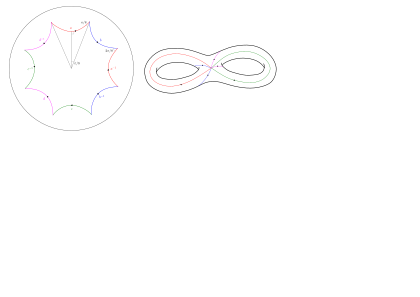
\includegraphics[width=1.0\textwidth]{figures/double_torus.png}
        \end{center}
        \caption{The identified octagonal polygon for the double torus in the
        Poincar\'e disc, and the corresponding cuts in the double torus.}
        \label{fig:double_torus}
    \end{figure}


    It is clear that with the given identification of the sides of $D$, the
    corresponding identified polygon $D^*$ is homeomorphic to $\Sigma_2$. This can
    also be shown by starting with a model of $\Sigma_2$, then introducing cuts to
    flatten it out. Since $D$ has finitely many sides, the conditions (a-g) are
    easily checked. Crucially, the cycle conditions work out because we are in the
    hyperbolic plane, where eight regular octagons can fit around a point.
    Poincar\'e's theorem now guarantees that $\mathbb{D}^2$ is indeed a universal
    cover of $\Sigma_2 \cong D^* \cong \mathbb{D}^2 / G$, where $G$ is the group
    generated by the cycle relations (there are no reflection relations here).
    Theorem.~\ref{th:group_quotient} also guarantees that the quotient map $p\colon
    \mathbb{D}^2 \to \Sigma_2$ is a normal covering space, that $G$ is the group of
    deck transformations of this covering space, and that $G \cong \pi_1(\Sigma_2)$.

    The space $\Sigma_2$ naturally inherits a differential structure from its
    universal cover $\mathbb{D}^2$; given $x \in \Sigma_2$, look at its pre-image in
    the fundamental octagon $\overline{D}$ and use the metric there. Note that there
    is no ambiguity, since the First Fundamental Form in $\mathbb{D}^2$ is identical
    for points the same distance from the origin, and $\pi^{-1}(x)$ consists of such
    radially symmetric points. Since the Poincar\'e disc has a constant negative
    curvature of $-1$, so does this model of $\Sigma_2$.


    \begin{figure}[H]
        \begin{center}
            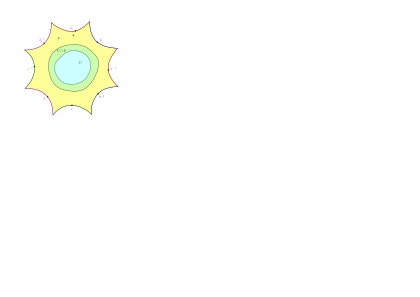
\includegraphics[width=0.7\textwidth]{figures/van_kampen.png}
        \end{center}
        \caption{Decomposing the double torus into two sets $U$ (cyan) and $V$
        (yellow), with their intersection $U \cap V$ (green). A loop
        travelling clockwise once in the green region can be pushed outwards to the
        boundary of the octagon.}
        \label{fig:van_kampen}
    \end{figure}


    We use Van Kampen's theorem to compute the fundamental group of $\Sigma_2$, by
    considering the two indicated open sets $U, V$ in $D^*$. Note that $U$ is
    contractible to a point hence its fundamental group is trivial. The set $V$
    deformation retracts to the boundary, which when properly identified consists of
    four loops sharing a single basepoint, i.e.\ the wedge product of four copies of
    $S^1$. Thus, the fundamental group of $V$ is the free group on four generators
    $a, b, c, d$.  Now, $U \cap V$ is an annulus which deformation retracts to a
    circle, hence has fundamental group $\Z$. The generator of $\pi_1(U \cap V)$, a
    single loop around the annulus in $U \cap V$, gets retracted to the boundary when
    viewed as a loop in $V$, hence corresponds to the homotopy class
    $[aba^{-1}b^{-1}cdc^{-1}d^{-1}] \in \pi_1(V)$. This loop must also correspond to
    the identity element in $\pi_1(U) = 0$, hence we have the relation
    $aba^{-1}b^{-1}cdc^{-1}d^{-1} = e$. Thus, we have \[
        \pi_1(\Sigma_2) = \langle a, b, c, d \mid
        aba^{-1}b^{-1}cdc^{-1}d^{-1}\rangle.
    \] This is isomorphic to the group $G$, and corresponds directly to its
    generators and cycle relations.


    \section{Conclusion}

    We have seen that it is possible to equip the topological manifold $\Sigma_2$
    with a differential structure giving it constant negative curvature $-1$. This is
    consistent with the Gauus-Bonnet formula \[
        \int_{\Sigma_g} K\:dA = 2\pi\chi(\Sigma_g) = 4\pi(1 - g).
    \] Note that plugging in $g = 2$ and $K = -1$ identically tells us that the total
    surface area of this structure is $4\pi$. Now, the area of each of the hyperbolic
    $(\pi / 2, \pi / 8, \pi / 8)$ triangles in the Poincar\'e disc, used in
    Figure.~3, is equal to the angle defect \[
        \pi - \left(\frac{\pi}{2} + \frac{\pi}{8} + \frac{\pi}{8}\right) =
        \frac{\pi}{4}.
    \] Since 16 of them combine to form our fundamental polygon, it has a total area
    of $4\pi$, as expected.

    We also note that the surfaces $\Sigma_g$ for genus $g \geq 3$ can also be
    constructed in a similar manner, by identifying the sides of a $4g$-gon with
    interior angles $2\pi / 4g$. The identification follows the same pattern as with
    the torus and the double torus. If we denote $[ab] = aba^{-1}b^{-1}$, then the
    sequence of identifications on the sides of the $4g$-gon read in order will be of
    the form $w = [a_1b_1][a_2b_2] \dots [a_g b_g]$. The fundamental group
    $\pi_1(\Sigma_g)$ can also be deduced as before, turning out to be the free group
    on the generators $a_1, b_1, \dots, a_g, b_g$ with the word $w$ as its only
    relation.


    \bibliographystyle{plain}
    \bibliography{references}
    \addcontentsline{toc}{section}{\numberline{}References}


\end{document}
